\def\documentauthor{Carlos Salinas}
\def\documenttitle{MA 166: Quiz {\hwnum} Solutions}
\def\hwnum{5}
\def\shorttitle{MA 166 HW {\hwnum} Solutions}
\def\coursename{MA166}
\def\documentsubject{calculus ii}
\def\authoremail{salinac@purdue.edu}

\documentclass[12pt]{article}
\usepackage{geometry}
\usepackage[dvipsnames]{xcolor}
\usepackage[
    breaklinks,
    bookmarks=true,
    % colorlinks=true,
    pageanchor=false,
    linkcolor=black,
    anchorcolor=black,
    citecolor=black,
    filecolor=black,
    menucolor=black,
    runcolor=black,
    urlcolor=black,
    hyperindex=false,
    hyperfootnotes=true,
    pdftitle={\shorttitle},
    pdfauthor={\documentauthor},
    pdfkeywords={\documentsubject},
    pdfsubject={\coursename}
    ]{hyperref}

% Use symbols instead of numbers
\renewcommand*{\thefootnote}{\fnsymbol{footnote}}

%% Math
\usepackage{amsmath}
\usepackage{amsthm}
\usepackage{amssymb}
\usepackage{mathtools}

%%PDFTeX specific
\usepackage[mathcal]{euscript}
\usepackage{mathrsfs}
\usepackage{dsfont}
\usepackage{wasysym}

\usepackage[LAE,LFE,T2A,T1]{fontenc}
\usepackage[utf8]{inputenc}
\usepackage[farsi,french,german,spanish,russian,english]{babel}
\babeltags{pa=farsi,
           fr=french,
           de=german,
           es=spanish,
           ru=russian,
           en=english}
\def\spanishoptions{mexico}

\selectlanguage{english}

\newcommand{\textfa}[1]{\beginR\textpa{#1}\endR}

\usepackage{cmap}
\usepackage{CJKutf8}
\newcommand{\textkr}[1]{\begin{CJK}{UTF8}{mj}#1\end{CJK}}
\newcommand{\textjp}[1]{\begin{CJK}{UTF8}{min}#1\end{CJK}}
\newcommand{\textzh}[1]{\begin{CJK}{UTF8}{bsmi}#1\end{CJK}}

%% Misc
\usepackage{graphicx}
\usepackage{cutwin}
\graphicspath{{figures/}}

\usepackage{microtype}
\usepackage{multicol}
\usepackage[inline]{enumitem}
\usepackage{listings}
\usepackage{mleftright}
\mleftright

%% Theorems and definitions
\theoremstyle{plain}
\newtheorem{theorem}{Theorem}
\newtheorem{proposition}[theorem]{Proposition}
\newtheorem{corollary}[theorem]{Corollary}
\newtheorem{claim}[theorem]{Claim}
\newtheorem{lemma}[theorem]{Lemma}
\newtheorem{axiom}[theorem]{Axiom}

\newtheorem*{corollary*}{Corollary}
\newtheorem*{claim*}{Claim}
\newtheorem*{lemma*}{Lemma}
\newtheorem*{proposition*}{Proposition}
\newtheorem*{theorem*}{Theorem}

\theoremstyle{definition}
\newtheorem{definition}{Definition}
\newtheorem{example}{Examples}
\newtheorem{examples}[example]{Examples}
\newtheorem{exercise}{Exercise}
\newtheorem{problem}[exercise]{Problem}

\newtheorem*{definition*}{Definition}
\newtheorem*{example*}{Examples}
\newtheorem*{examples*}{Examples}
\newtheorem*{exercise*}{Exercise}
\newtheorem*{problem*}{Problem}

\theoremstyle{remark}
\newtheorem{remark}{Remark}
\newtheorem{remarks}[remark]{Remarks}
\newtheorem{observation}[remark]{Observation}
\newtheorem{observations}[remark]{Observations}

\newtheorem*{remark*}{**Remark**}
\newtheorem*{remarks*}{**Remarks**}
\newtheorem*{observation*}{**Observation**}
\newtheorem*{observations*}{**Observations**}

%% Commands and operators
%% Redefinitions & commands
\newcommand{\nsubset}{\ensuremath{\not\subset}}
\newcommand{\nsupset}{\ensuremath{\not\supset}}
\newcommand\minus{\ensuremath{\null\smallsetminus}}
\renewcommand\qedsymbol{\ensuremath{\null\hfill\smiley}}

%% Commands and operators
\DeclareMathOperator{\id}{id}
\DeclareMathOperator{\im}{im}

%% Linear algebra
\DeclareMathOperator{\proj}{proj}
\DeclareMathOperator{\comp}{comp}

%% Differential operators
\DeclareMathOperator{\Curl}{curl}
\DeclareMathOperator{\Div}{div}
\DeclareMathOperator{\Grad}{grad}
\DeclareMathOperator{\Lap}{\Delta}
\DeclareMathOperator{\diff}{d\!}

%% Misc
\newcommand{\bbC}{\mathbb{C}}
\newcommand{\bbCP}{\mathbb{CP}}
\newcommand{\bbH}{\mathbb{H}}
\newcommand{\bbN}{\mathbb{N}}
\newcommand{\bbQ}{\mathbb{Q}}
\newcommand{\bbR}{\mathbb{R}}
\newcommand{\bbRP}{\mathbb{RP}}
\newcommand{\bbZ}{\mathbb{Z}}

\newcommand{\bfC}{\mathbf{C}}
\newcommand{\bfCP}{\mathbf{CP}}
\newcommand{\bfH}{\mathbf{H}}
\newcommand{\bfN}{\mathbf{N}}
\newcommand{\bfQ}{\mathbf{Q}}
\newcommand{\bfR}{\mathbf{R}}
\newcommand{\bfRP}{\mathbf{RP}}
\newcommand{\bfZ}{\mathbf{Z}}

\newcommand{\calA}{\mathcal{A}}
\newcommand{\calB}{\mathcal{B}}
\newcommand{\calC}{\mathcal{C}}
\newcommand{\calS}{\mathcal{S}}
\newcommand{\calT}{\mathcal{T}}
\newcommand{\calU}{\mathcal{U}}
\newcommand{\calV}{\mathcal{V}}

\newcommand{\scrL}{\mathscr{L}}
\newcommand{\scrO}{\mathscr{O}}
\newcommand{\scrS}{\mathscr{S}}

\newcommand{\bfa}{\mathbf{a}}
\newcommand{\bfb}{\mathbf{b}}
\newcommand{\bfc}{\mathbf{c}}
\newcommand{\bfu}{\mathbf{u}}
\newcommand{\bfv}{\mathbf{v}}
\newcommand{\bfw}{\mathbf{w}}

\begin{document}
\author{TA: \href{mailto:\authoremail}{\documentauthor}}
\title{\documenttitle}
\date{\today}
\maketitle

You have \textbf{15 minutes} to complete this quiz. You may work in groups,
but you are not allowed to use any other resources.
\\\\
\begin{problem}
Evaluate the integral
\[
\int_0^{\pi/2}\cos^2x\;dx.
\]
\end{problem}
\bigskip
\begin{problem}
Evaluate the integral
\[
\int\frac{x^2}{\sqrt{4-x^2}}\;dx.
\]
(Use $C$ for the constant of integration.)
\end{problem}
\bigskip
\begin{problem}
Evaluate the integral
\[
\int\frac{e^x}{1-e^{2x}}\;dx
\]
[\textsc{Hint:} First use a substitution and then partial fractions.]
\end{problem}
\newpage
\section*{Solutions}
\begin{proof}[Solution to Problem 1]
Use the double-angle identity
\begin{equation}
\label{eq:cos-double-angle}
\cos^2\theta=\frac{1+\cos2\theta}{2}
\end{equation}
to rewrite the integral
\begin{align*}
\int_0^{\pi/2}\cos^2 x\;dx
&=\int_0^{\pi/2}\frac{1+\cos2x}{2}\;dx\\
&=\frac{1}{2}\int_0^{\pi/2}1+\cos2x\;dx\\
&=\frac{1}{2}\int_0^{\pi/2}1\;dx+\frac{1}{2}\int_0^{\pi/2}\cos 2x\;dx\\
&=\frac{1}{2}\left(\left.x\right|_0^{\pi/2}\right)
+\frac{1}{2}\left(\left.\frac{\sin 2x}{2}\right|_0^{\pi/2}\right)\\
&=\frac{1}{2}\left(\frac{\pi}{2}-0\right)+\frac{1}{2}\left(\frac{1}{2}\sin
  \pi-\frac{1}{2}\sin 2\cdot 0\right)\\
&=\frac{1}{2}\left(\frac{\pi}{2}-0\right)+\frac{1}{2}\left(0-0\right)\\
&=\frac{1}{2}\frac{\pi}{2}+\frac{1}{2}\cdot 0\\
&=\boxed{\frac{\pi}{4}.}\qedhere
\end{align*}
\end{proof}

\begin{proof}[Solution to Problem 2]
Since we have something of the form $\sqrt{4-x^2}$ in the denominator, the
best approach to this problem is to make a trigonometric substitution. Draw
the triangle
\begin{equation}
\label{eq:trig-subst}
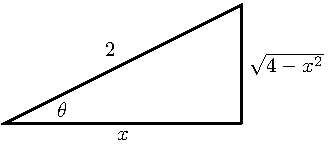
\includegraphics{../figures/qiz-5-triangle}
\end{equation}
from which we can deduce that
\begin{equation}
\label{eq:trig-subst}
\cos\theta=\frac{x}{2}\qquad\qquad
\sin\theta=\frac{\sqrt{4-x^2}}{2}.
\end{equation}
Hence, $2\cos\theta=x$ and $-2\sin\theta\;d\theta=dx$ so substituting this
into our original integral, we have
\begin{align*}
\int\frac{x^2}{\sqrt{4-x^2}}\;dx
&=\int\frac{(2\cos\theta)^2}{2\sin\theta}(-2\sin\theta)\;d\theta\\
&=-4\int\cos^2\theta\;d\theta\\
\intertext{here, using the double-angle formula
  \eqref{eq:cos-double-angle}, we have}
&=-4\int\frac{1}{2}\left(1+\cos2\theta\right)\;d\theta\\
&=-2\int 1+\cos2\theta\;d\theta\\
&=-2\int 1\;d\theta+\int \cos2\theta\;d\theta\\
&=-2\theta-2\left(\frac{1}{2}\sin 2\theta\right)+C\\
&=-2\theta-\sin 2\theta+C.
\end{align*}
Substituting back in, we have
\[
\theta=\cos^{-1}(x/2)
\]
and
\[
\sin2\theta=2\cos\theta\sin\theta=
2\left(\frac{x}{2}\right)
\left(\frac{\sqrt{4-x^2}}{2}\right)=
\frac{x\sqrt{4-x^2}}{2}
\]
so our integral is
\[
\boxed{-2\cos^{-1}(x/2)-\frac{x\sqrt{4-x^2}}{2}+C.}
\]
\textbf{Note} that if you used a different substitution, say you labeled
the adjacent side with $\sqrt{4-x^2}$, then $\sin\theta=x/2$ and you would
get
\[
\boxed{2\sin^{-1}\left(\frac{x}{2}\right)-\frac{x\sqrt{4-x^2}}{2}+C'}
\]
where $C'=C-\pi$. This is because $\cos^{-1}\theta=\pi/2-\sin^{-1}\theta$.
\end{proof}

\begin{proof}[Solution to Problem 3]
Make the substitution $u=e^x$, then $du=e^x\;dx=u\;dx$ and our integral
turns into
\begin{align*}
\int\frac{e^x}{1-e^{2x}}\;dx
&=\int\frac{u}{1-u^2}\frac{du}{u}\\
&=\int\frac{1}{1-u^2}\;du\\
&=\int\frac{1}{(1-u)(1+u)}\;du.
\end{align*}
Now we find the partial fraction decomposition
\[
\frac{1}{(1-u)(1+u)}=\frac{A}{1-u}+\frac{B}{1+u}
\]
so, clearing denominators, we have
\[
1=A(1+u)+B(1-u)=(A-B)u+A+B.
\]
so we must have $A-B=0$ and $A+B=1$. This tells us that $A=B$ so
substituting this into the former equation $A+B=A+A=2A=1$ so
$A=B=1/2$. Hence, our integral turns into
\begin{align*}
\int\frac{1}{(1-u)(1+u)}\;du
&=\frac{1}{2}\int\frac{1}{1-u}+\frac{1}{1+u}\;du\\
&=\frac{1}{2}\int\frac{1}{1-u}\;du
+\frac{1}{2}\int\frac{1}{1+u}\;du\\
&=-\frac{1}{2}\ln|1-u|+\frac{1}{2}\ln|1+u|+C\\
\intertext{substituting back our value of $u$, we have}
&=-\frac{1}{2}\ln|1-u|+\frac{1}{2}\ln|1+u|+C\\
&=\boxed{
-\frac{1}{2}\ln\left|1-e^x\right|
+\frac{1}{2}\ln\left|1+e^x\right|+C.}
\end{align*}
\textbf{Note} that this problem can also be done using a trig
substitution. Looking back at the original integral after we made a
substitution
\[
\int\frac{1}{1-u^2}\;du
=\int\frac{1}{\left(\sqrt{1-u^2}\right)^2}\;du
\]
and making the trig substitution $\cos\theta=x$, $-\sin\theta\;d\theta=dx$
we have
\begin{align*}
\int\frac{1}{\left(\sqrt{1-u^2}\right)^2}\;du
&=\int\frac{-\sin\theta}{\sin^2\theta}\;d\theta\\
&=-\int\csc\theta\;d\theta\\
&=-\ln\left|\csc\theta-\cot\theta\right|+C\\
\intertext{where $\csc\theta=1/\sqrt{1-u^2}$ and
  $\cot\theta=u/\sqrt{1-u^2}$ so}
&=-\ln\left|\csc\theta-\cot\theta\right|+C\\
&=-\ln\left|\frac{1}{\sqrt{1-u^2}}-\frac{u}{\sqrt{1-u^2}}\right|+C\\
&=-\ln\left|\frac{1-u}{\sqrt{1-u^2}}\right|+C\\
&=-\ln\left|\frac{1-u}{\sqrt{1-u^2}}\right|+C\\
\intertext{by properties of the logarithm, namely, $\ln(a/b)=\ln a-\ln b$,
  we have }
&=-\ln\left|1-u\right|+\ln\left|\sqrt{1-u^2}\right|+C\\
&=-\ln\left|1-u\right|+\frac{1}{2}\ln\left|1-u^2\right|+C\\
&=-\ln\left|1-u\right|+\frac{1}{2}\ln\left|(1-u)(1+u)\right|+C\\
&=-\ln\left|1-u\right|+\frac{1}{2}\ln\left|1-u\right|
+\frac{1}{2}\ln\left|(1+u)\right|+C\\
&=-\frac{1}{2}\ln\left|1-u\right|+\frac{1}{2}\ln\left|1-u\right|+C\\
\intertext{lastly, we substitute our original value of $u$}
&=\boxed{-\frac{1}{2}\ln\left|1-e^x\right|+\frac{1}{2}\l\left|1+e^x\right|+C.}
\qedhere
\end{align*}
This integral was much tougher to compute than the partial fractions as it
required you to know the integral of $\csc\theta$ (or $\sec\theta$ if your
trig substitution was $\sin\theta=x$), which is why I wanted you to do the
partial fractions. Still, some students took this approach. There's more
than one way to skin a cat, I suppose.
\end{proof}
\end{document}

%%% Local Variables:
%%% mode: latex
%%% TeX-master: t
%%% End:
